\documentclass[border=8pt]{standalone}
\usepackage{tikz}
\usetikzlibrary{arrows.meta,shapes.geometric}
\pdfmapfile{+cm.map}
\begin{document}
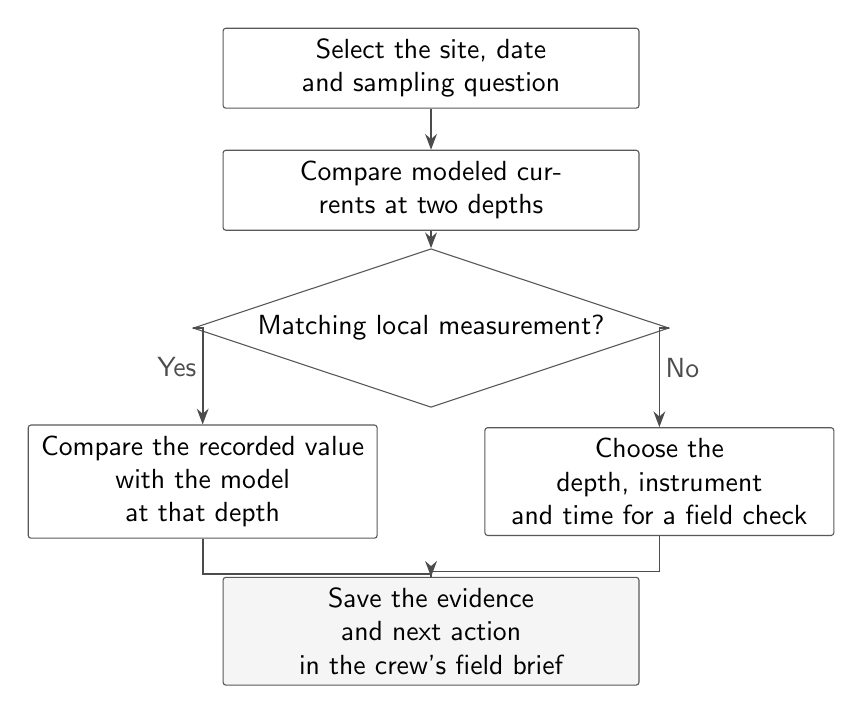
\begin{tikzpicture}[x=1cm,y=1cm, font=\sffamily, box/.style={draw=black!65,rounded corners=1pt,align=center,minimum height=0.83cm,text width=5.0cm,inner sep=4pt}, edge/.style={-{Stealth[length=2mm]},semithick,black!70}]
\node[box] (target) at (0,0) {Select the site, date and sampling question};
\node[box] (model) at (0,-1.55) {Compare modeled currents at two depths};
\node[draw=black!65,diamond,aspect=3,align=center,inner sep=2.5pt] (gate) at (0,-3.3) {Matching local measurement?};
\node[box,text width=4.15cm] (obs) at (-2.9,-5.25) {Compare the recorded value\\with the model at that depth};
\node[box,text width=4.15cm] (req) at (2.9,-5.25) {Choose the depth, instrument\\and time for a field check};
\node[box,fill=black!4] (out) at (0,-7.15) {Save the evidence and next action\\in the crew's field brief};
\draw[edge] (target)--(model);
\draw[edge] (model)--(gate);
\draw[edge] (gate.west) -| node[pos=.7,left,fill=white,inner sep=2pt]{Yes} (obs.north);
\draw[edge] (gate.east) -| node[pos=.7,right,fill=white,inner sep=2pt]{No} (req.north);
\draw[edge] (obs.south) -- ++(0,-.45) -| (out.north);
\draw[semithick,black!70] (req.south) -- ++(0,-.45) -| (out.north);
\end{tikzpicture}
\end{document}
